\section{[WIP]Benutzerf"uhrung}

\subsection{Elemente der grafischen Benutzeroberfl"ache}

\begin{figure}[htb]
\centering
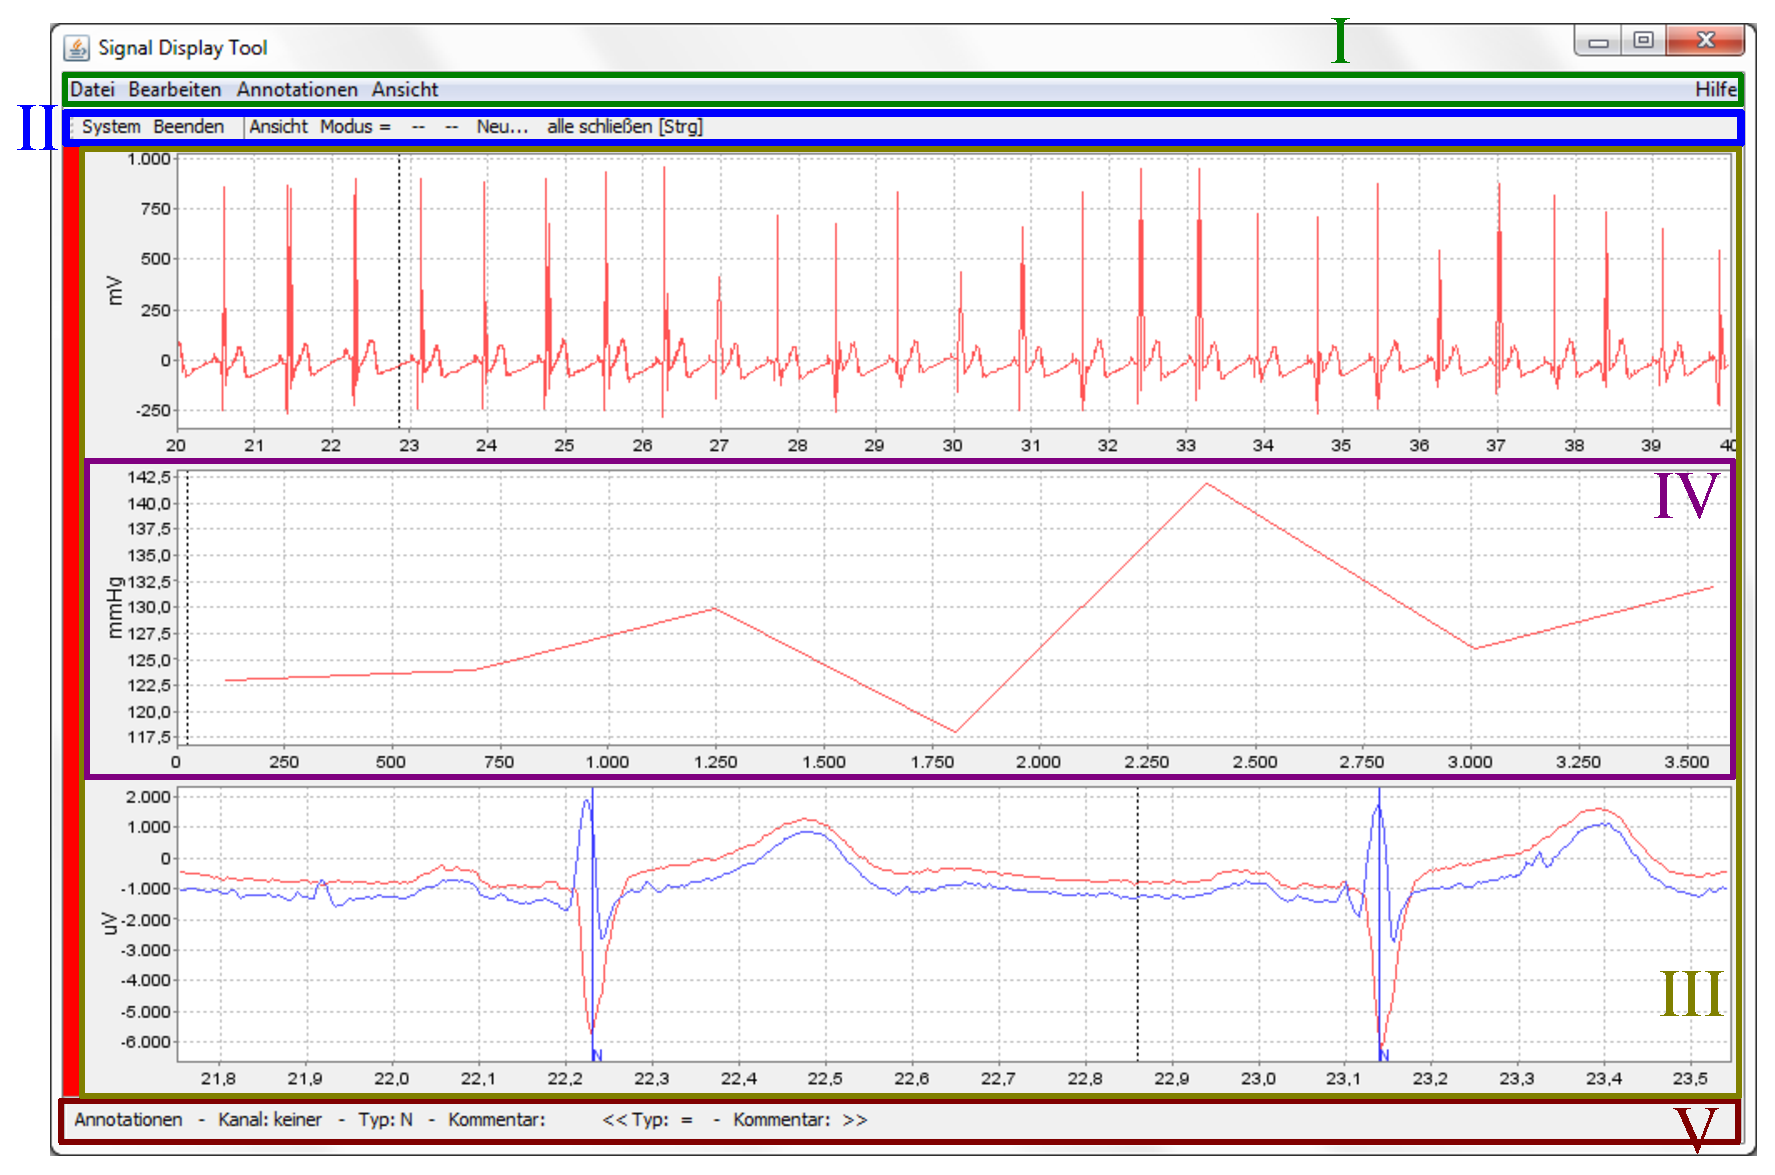
\includegraphics[width=\textwidth]{bilder/programm_ansicht.eps}
\caption[Klassen der grafischen Elemente]{Klassen der grafischen Elemente: I \texttt{Menus}, II \texttt{Toolbar}, III \texttt{SignalPanel}, IV \texttt{SignalView}, V \texttt{StatusBar}}
\label{pic:gui_elements_and_classes}
\end{figure}

In \picref{gui_elements_and_classes} sind die einzelnen Bestandteile der \ac{GUI} hervorgehoben.
Interaktionen zwischen dem Benutzer und dem Programm erfolgen "uber f"unf Hauptkomponenten:
\begin{itemize}
	\item Men"uzeile durch die Klasse \class{Menus} repr"asentiert
	\item Werkzeugleiste als Klasse \class{Toolbar}
	\item Statuszeile zum Anzeigen von Informationen mithilfe der Klasse \class{StatusBar}
	\item einzelne Diagramme als \class{SignalView}s zur Anzeige der Signalverl"aufe (im folgendem Signalansichten genannt)
	\item Zusammenfassung aller Signalansichten auf dem fl"achengr"o{\ss}tem Bestandteil, dem \class{SignalPanel}
\end{itemize}
W"ahrend das Men"u, die Werkzeugleiste und die Signalansichten Eingaben von dem Benutzer verarbeiten, dient die Statuszeile ausschlie{\ss}lich der Pr"asentation von Informationen.
Die grafische Darstellung der Klasse \class{SignalPanel} bleibt f"ur den Nutzer gr"o{\ss}tenteils verborgen, da es sich hierbei um ein organisatorisches Programmelement handelt (siehe dazu \secref{signalpanel_organisation}).

\begin{figure}[htb]
\centering
\includegraphics[angle=-90, width=0.9\textwidth]{bilder/package_ui_ubersicht.pdf}
\caption{"Ubersicht "uber das \class{ui}-Paket}
\label{pic:package_ui_ubersicht}
\end{figure}

Ein "Ubersicht die Klassenhierarchie ist in \picref{package_ui_ubersicht} dargestellt.
Bis auf die \class{SignalView}-Klasse sind alle grafischen Komponenten nach dem Singleton-Entwurfsmuster implementiert (vgl. \secref{singleton}).
Durch diese Entscheidung ist einerseits garantiert, dass die grafischen Elemente nur einmal in der Programminstanz vorkommen und au{\ss}erdem kann auf sie vereinfacht zugegriffen werden ("ahnlich wie auf globale Variablen).

%- alle Elemente Singleton (bis auf \class{SignalView})

\subsection{[WIP]Visualisierung der Signalverl"aufe}

- Nutzung von JFreeChart (\ac{lgpl})
- langsam bei der darstellung vieler Datenpunkte
- Einschr"ankung durch begrenzung der Punkte auf die Pixelbreite des entsprechenden Diagramms
- Klasse \class{SignalView}

\subsection{[WIP]Gr"o{\ss}enbestimmung und Positionierung der Signalansichten durch \class{SignalPanel}}
\label{sec:signalpanel_organisation}

- organisationseinheit

\subsection{[WIP]Verarbeitung der Benutzereingabe im Paket \class{ui}}


\subsubsection{[WIP]Koordiniertes Zoomen und Scrollen durch \class{SignalPanel}}

- Observer-Prinzip
- zwei eigene Managerklassen (Unabh"angigkeit) \class{ScrollLockManager}, \class{ZoomLockManager}

\subsubsection{[WIP]Darstellung und Verarbeitung der Benutzereingaben}

- \class{SignalView} stellt dar
- Datenzugriff "uber abstrakte Definition von \class{DataController}
- Subklassen verarbeiten Maus- und Tastatureingabe

\subsubsection{[WIP]Verarbeitung und Ver"anderung von Annotationen}

- Einf"ugen von Annotationen "uber \class{AnnotationManager}
- Dreiecksbeziehung von \class{Annotation\-Controller}, \class{AnnotationList} und \class{AnnotationManager} erl"autern
- Suchalgorithmus zum finden der aktuellen Annotation
- "Anderung wird durch die Implementierung vom Interface \class{Data\-Change\-Listener} automatisiert aktualisiert

% EOF
